
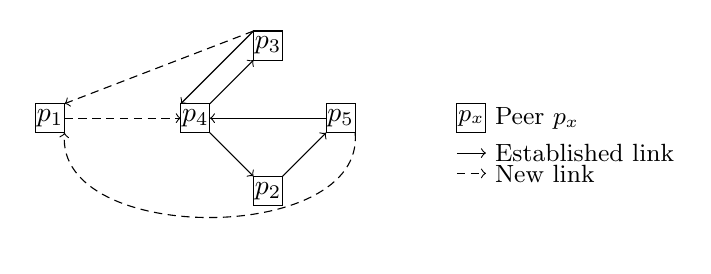
\begin{tikzpicture}[scale=1.05]
  
  \draw[fill=white] (0pt, 0pt) node{$p_1$} +(-5pt,-5pt) rectangle +(5pt,5pt);

  \begin{scope}[shift={(75pt,0pt)}]
  \draw[fill=white] (0pt, -25pt) node{$p_2$} +(-5pt,-5pt) rectangle +(5pt,5pt);
  \draw[fill=white] (0pt,  25pt) node{$p_3$} +(-5pt,-5pt) rectangle +(5pt,5pt);
  \draw[fill=white] (-25pt, 0pt) node{$p_4$} +(-5pt,-5pt) rectangle +(5pt,5pt);
  \draw[fill=white] ( 25pt, 0pt) node{$p_5$} +(-5pt,-5pt) rectangle +(5pt,5pt);

  \draw[->] (-20pt, 5pt) -- (-5pt, 20pt); %% u4 -> u3
  \draw[->] (-20pt,-5pt) -- (-5pt,-20pt); %% u4 -> u2
  \draw[->] ( 5pt,-20pt) -- (20pt, -5pt); %% u2 -> u5
  \draw[->] (20pt,  0pt) -- (-20pt, 0pt); %% u5 -> u4
  \draw[->] (-5pt, 30pt) -- (-30pt, 5pt); %% u3 -> u4

  \draw[->, densely dashed] (-70pt, 0pt) -- (-30pt, 0pt); %% u1 -> u4
  \draw[->, densely dashed] (-5pt, 30pt) -- (-70pt, 5pt); %% u3 -> u1
  \draw[->, densely dashed] (30pt, -5pt) to[out=-85,in=-95](-70pt,-5pt);%%u5 u1
  \end{scope}
  
  \small 
  \begin{scope}[shift={(140pt,0pt)}]
    \draw[fill=white](5pt, 0pt)node{$p_x$}+(-5pt,-5pt) rectangle +(5pt,5pt);
    \draw (10pt,0pt) node[anchor=west]{Peer $p_x$};
    \draw[->](0pt, -12pt)--(10pt, -12pt) node[anchor=west]{Established link};
    \draw[->, densely dashed](0pt, -19pt)--(10pt, -19pt)
    node[anchor=west]{New link};
    
  \end{scope}
  
\end{tikzpicture}